% Straight up stealing preamble from Eli Holmes 
%%%%%%%%%%%%%%%%%%%%%%%%%%%%%%%%%%%%%%START PREAMBLE THAT IS THE SAME FOR ALL EXAMPLES
\documentclass{article}

%Required: You must have these
\usepackage{Sweave}
\usepackage{graphicx}
\usepackage{tabularx}
\usepackage{hyperref}
\usepackage{natbib}
\usepackage{pdflscape}
\usepackage{array}
\usepackage{gensymb}
%\usepackage[backend=bibtex]{biblatex}
%Strongly recommended
  %put your figures in one place
%\SweaveOpts{prefix.string=figures/, eps=FALSE} 
%you'll want these for pretty captioning
\usepackage[small]{caption}

\setkeys{Gin}{width=0.8\textwidth}  %make the figs 50 perc textwidth
\setlength{\captionmargin}{30pt}
\setlength{\abovecaptionskip}{10pt}
\setlength{\belowcaptionskip}{10pt}
% manual for caption  http://www.dd.chalmers.se/latex/Docs/PDF/caption.pdf

%Optional: I like to muck with my margins and spacing in ways that LaTeX frowns on
%Here's how to do that
 \topmargin -1.5cm        
 \oddsidemargin -0.04cm   
 \evensidemargin -0.04cm  % same as oddsidemargin but for left-hand pages
 \textwidth 16.59cm
 \textheight 21.94cm 
 %\pagestyle{empty}       % Uncomment if don't want page numbers
 \parskip 7.2pt           % sets spacing between paragraphs
 %\renewcommand{\baselinestretch}{1.5} 	% Uncomment for 1.5 spacing between lines
\parindent 0pt% sets leading space for paragraphs
\usepackage{setspace}
%\doublespacing

%Optional: I like fancy headers
%\usepackage{fancyhdr}
%\pagestyle{fancy}
%\fancyhead[LO]{How do climate change experiments actually change climate}
%\fancyhead[RO]{2016}
 
%%%%%%%%%%%%%%%%%%%%%%%%%%%%%%%%%%%%%%END PREAMBLE THAT IS THE SAME FOR ALL EXAMPLES

%Start of the document
\begin{document}

%\SweaveOpts{concordance=TRUE}
 \bibliographystyle{/Users/aileneettinger/citations/Bibtex/styles/amnat.bst}
\title{Spatial and temporal shifts in photoperiod with climate change} % perspective paper for OSPREE analyses

\author{A.K. Ettinger, C. Adams, D. Buonaiuto, I. Morales Castilla, E. Wolkovich}
%\date{\today}
\maketitle  %put the fancy title on
%\tableofcontents      %add a table of contents
%\clearpage
%%%%%%%%%%%%%%%%%%%%%%%%%%%%%%%%%%%%%%%%%%%%%%%%%%%

\section* {Spatial and temporal shifts in photoperiod with climate change}
\par Problem: Shifts in temperature (warming) and, to a lesser extent, precipitation, have been the focus of studies seeking to document biological impacts of climate change and to forecast future impacts under additional change. Photoperiod is another critical cue used by organisms, and it will also be altered by climate change. It has been argued that “Day length is the most...consistent environmental cue in northernmost seasonal environments." Yet, as species undergo climate change-induced shifts in space and/or time, the the daylength they experience will be altered. The biological implications of these altered photoperiods, and how they will interact with other environmental cues, are not well understood.

General points/questions to address:

How will climate change alter the photoperiod experienced by organisms?

    If a species shift up in latitude (as many already have, and as is forecasted), organisms will experience altered photoperiods. For example, on May 15, the day length is 14 hours in Washington, DC. On the same date, the day length in Montreal (about 6 degrees poleward in latitude) is an hour longer. (Prior to the spring equinox, around March 20, Montreal would have shorter daylengths than Washington DC). Species are moving at a rate of ~6km ( or ~0.05 degrees) per decade poleward (Parmesan 2006), so a species might experience this shift in photoperiod in ~1000 years.

    If a species shifts earlier temporally (as many already have, and as is forecasted), organisms will also experience altered photoperiod, but not necessarily in the same direction. For example, in Washington DC, the daylength on April 15 is about 1 hour shorter than on May 15. Species are shifting phenology at a rate of 3-5 days earlier per decade (Parmesan 2006), so a species might experience this shift in photoperiod in ~100 years.

    Therefore, given previous rates of temporal and spatial shifts in species, a species that currently leafs out in Washington DC on May 15 will experience longer day length on this day, if its range shifts up in latitude to match the climate niche of its current location. On the other hand, if it stayed in Washington, DC and shifted its phenology earlier, it would experience shorter daylengths. (Include a figure and/or map of these differences)

Implications of shifts in photoperiod

    Interactions between photoperiod and forcing and chilling could result in muted or exaggerated phenological shifts, compared to what would be expected based on temperature change alone.
. 
%\bibliography{/Users/aileneettinger/citations/Bibtex/mylibrary}
\clearpage

\section* {Figures}
\begin{figure}[p]
\centering
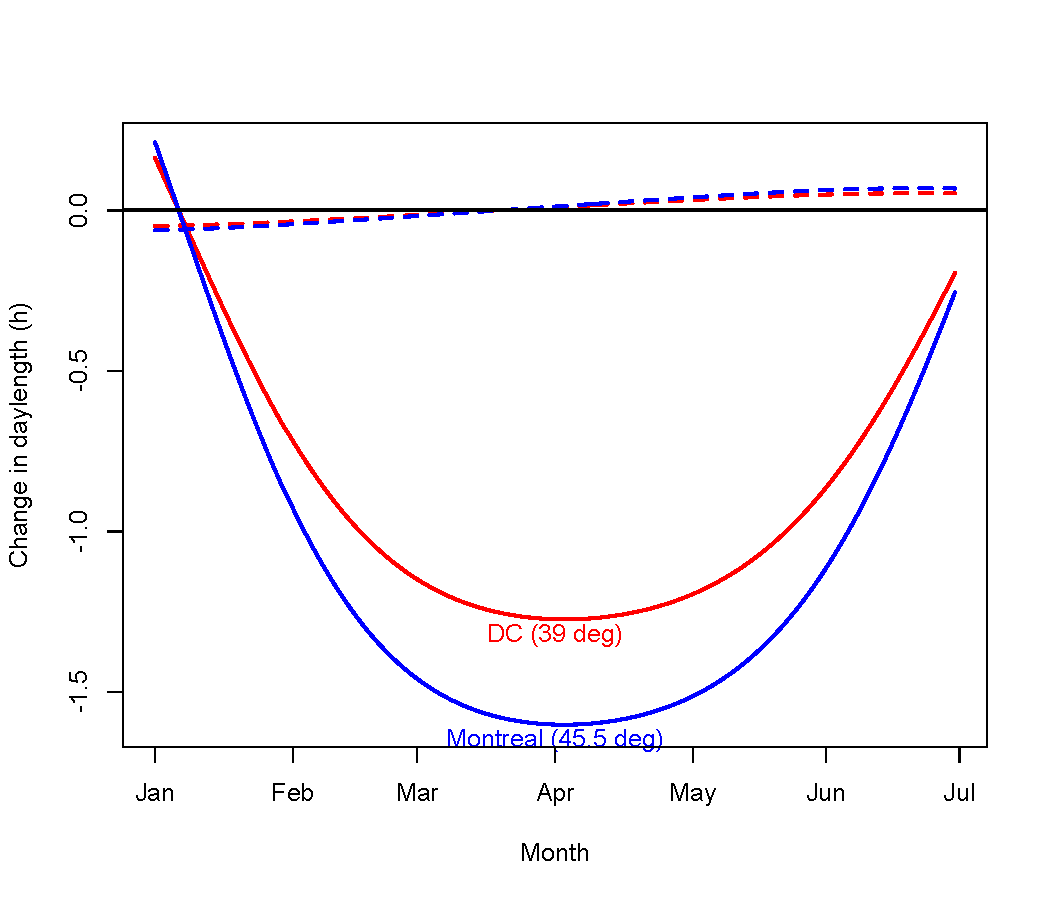
\includegraphics{/Users/aileneettinger/git/ospree/analyses/figures/photoper_change.pdf} 
\caption{\textbf{Shifts in the photoperiod organisms will experience with climate change, at two latitudes (Washington, DC and Montreal).}  With warming, species are likely to shift their ranges poleward and/or shift their spring activity earlier, resulting in alterations to the photoperiod they experience. We compare changes to photoperiod in 100 years if species shift spatially (solidi.e. shifting their ranges ~6km,or 0.05 degree, per decade poleward, solid lines) versus temporally (shifting activity earlier 3 days per decade, dashed lines).}
 \label{fig:photo}
 \end{figure}
\begin{figure}[p]
\centering
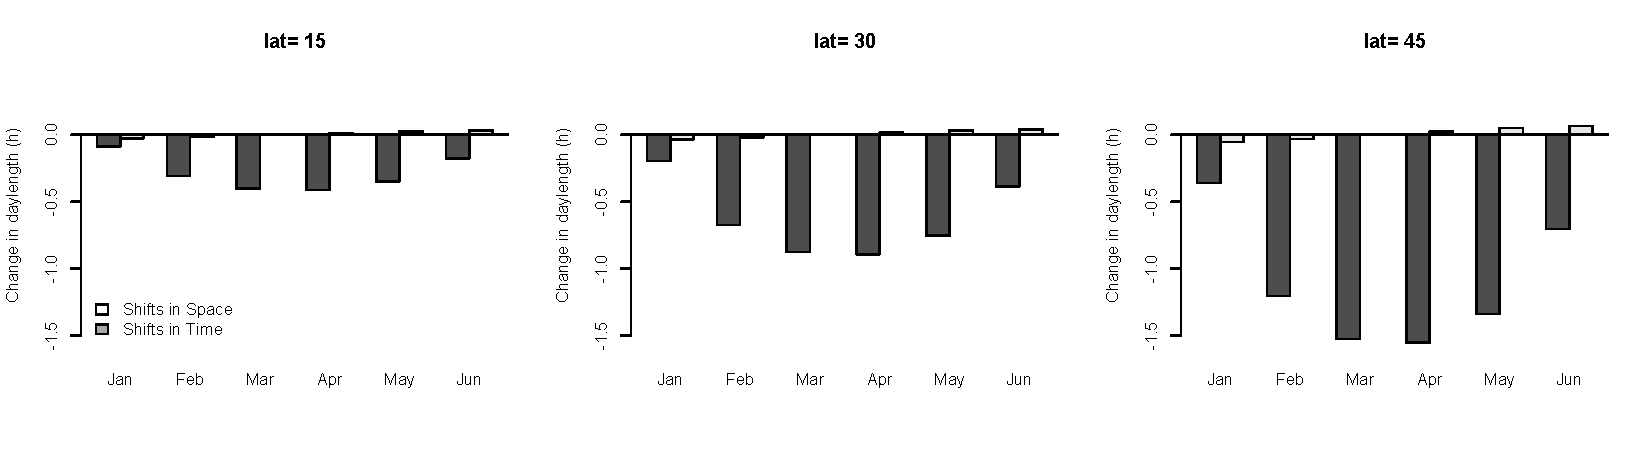
\includegraphics{/Users/aileneettinger/git/ospree/analyses/figures/photoper_change_bar.pdf} 
\caption{\textbf{Shifts in the photoperiod organisms will experience with climate change, across latitude.}  With warming, species are likely to shift their ranges poleward and/or shift their spring activity earlier, resulting in alterations to the photoperiod they experience. We compare changes to photoperiod in 100 years if species shift spatially (i.e. shifting their ranges ~6km,or 0.05 degree, per decade poleward) versus temporally (shifting activity earlier 3 days per decade).}
 \label{fig:photo}
 \end{figure}
\clearpage



%%%%%%%%%%%%%%%%%%%%%%%%%%%%%%%%%%%%%%%%
\end{document}
%%%%%%%%%%%%%%%%%%%%%%%%%%%%%%%%%%%%%%%%
